\documentclass{article}
\usepackage{amsmath,amssymb,amsthm,mdframed,kotex,paralist}
\usepackage{tabto}
%\TabPositions{0.5\textwidth}
\TabPositions{0.33\textwidth,0.66\textwidth}
\newcommand\bp[1]{\begin{mdframed}[frametitle={#1},skipabove=10pt,skipbelow=20pt,innertopmargin=5pt,innerbottommargin=40pt]}
\newcommand\ep{\end{mdframed}\par}

\begin{document}
\title{준형03}
\author{}
\date{\today}
\maketitle
%\section{이차함수의 개형}

\bp{01}
다음 그림과 같은 직사각형 ABCD에서 점 \(G\)가 \(\overline{EF}\) 위에서 움직일 때 직사각형 BHGI의 넓이의 최대값은?
(단 모눈 한 개의 눈금은 1이다.)
\par\medskip
\begin{center}
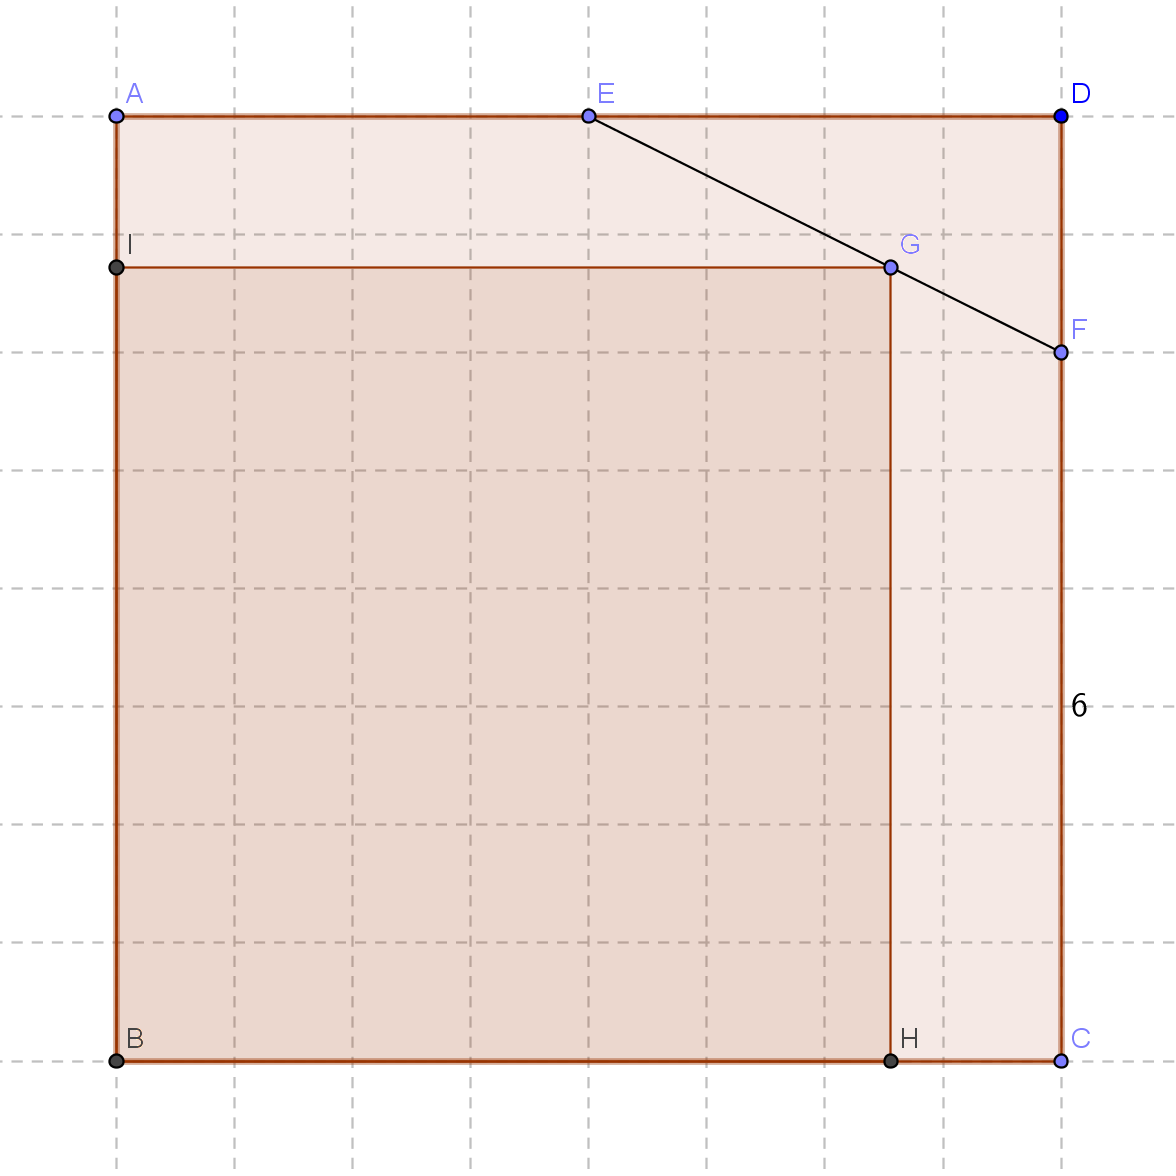
\includegraphics[width=0.7\textwidth]{problem_01}
\end{center}\medskip
\ep

\bp{02}
다음 그림과 같은 직사각형 ABCD에서 점 \(G\)가 \(\overline{EF}\) 위에서 움직일 때 직사각형 BHGI의 넓이의 최대값은?
(단 모눈 한 개의 눈금은 1이다.)
\par\medskip
\begin{center}
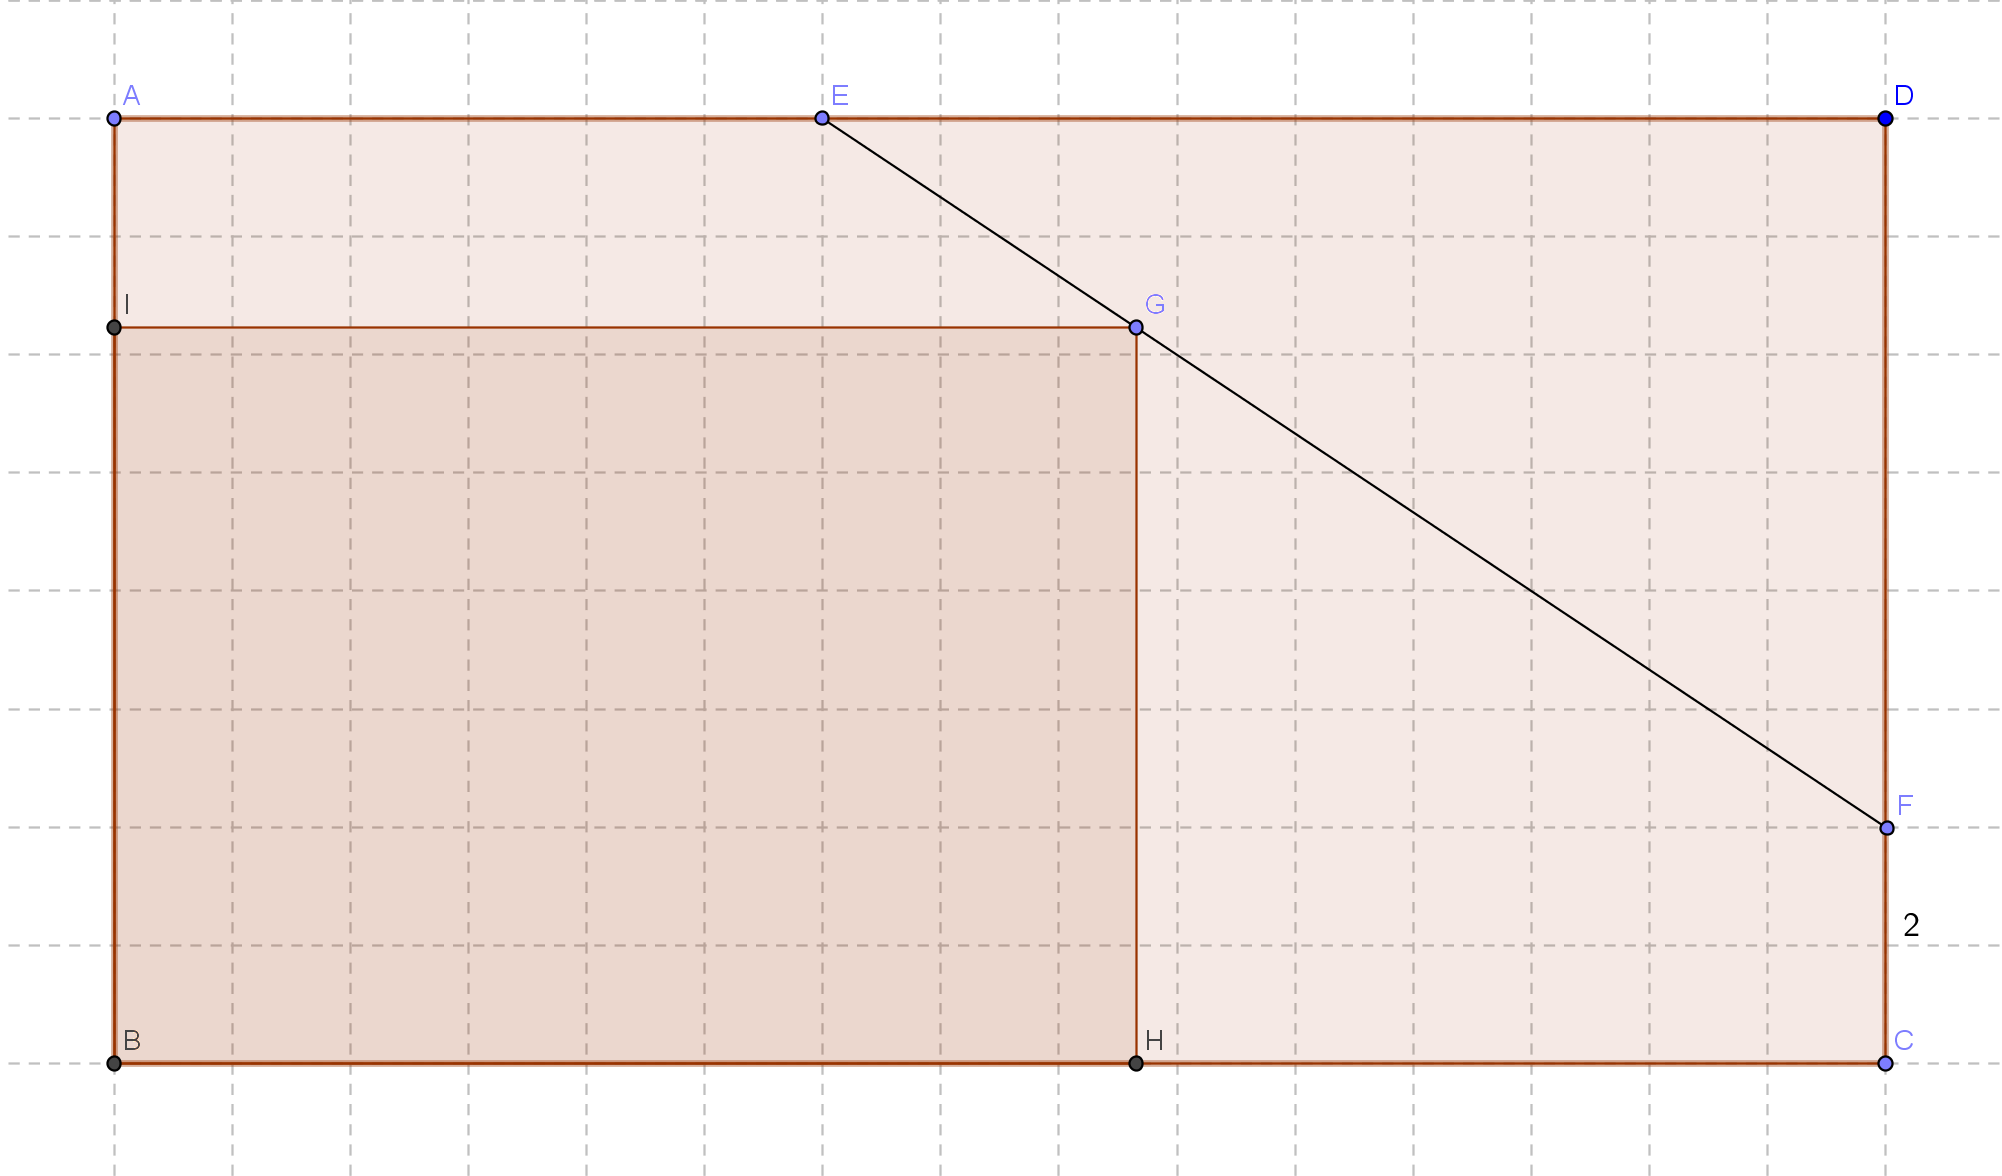
\includegraphics[width=0.7\textwidth]{problem_02}
\end{center}\medskip
\ep

\bp{03}
다음 그림과 같은 직사각형 ABCD에서 점 \(G\)가 \(\overline{EF}\) 위에서 움직일 때 직사각형 BHGI의 넓이의 최대값은?
(단 모눈 한 개의 눈금은 1이다.)
\par\medskip
\begin{center}
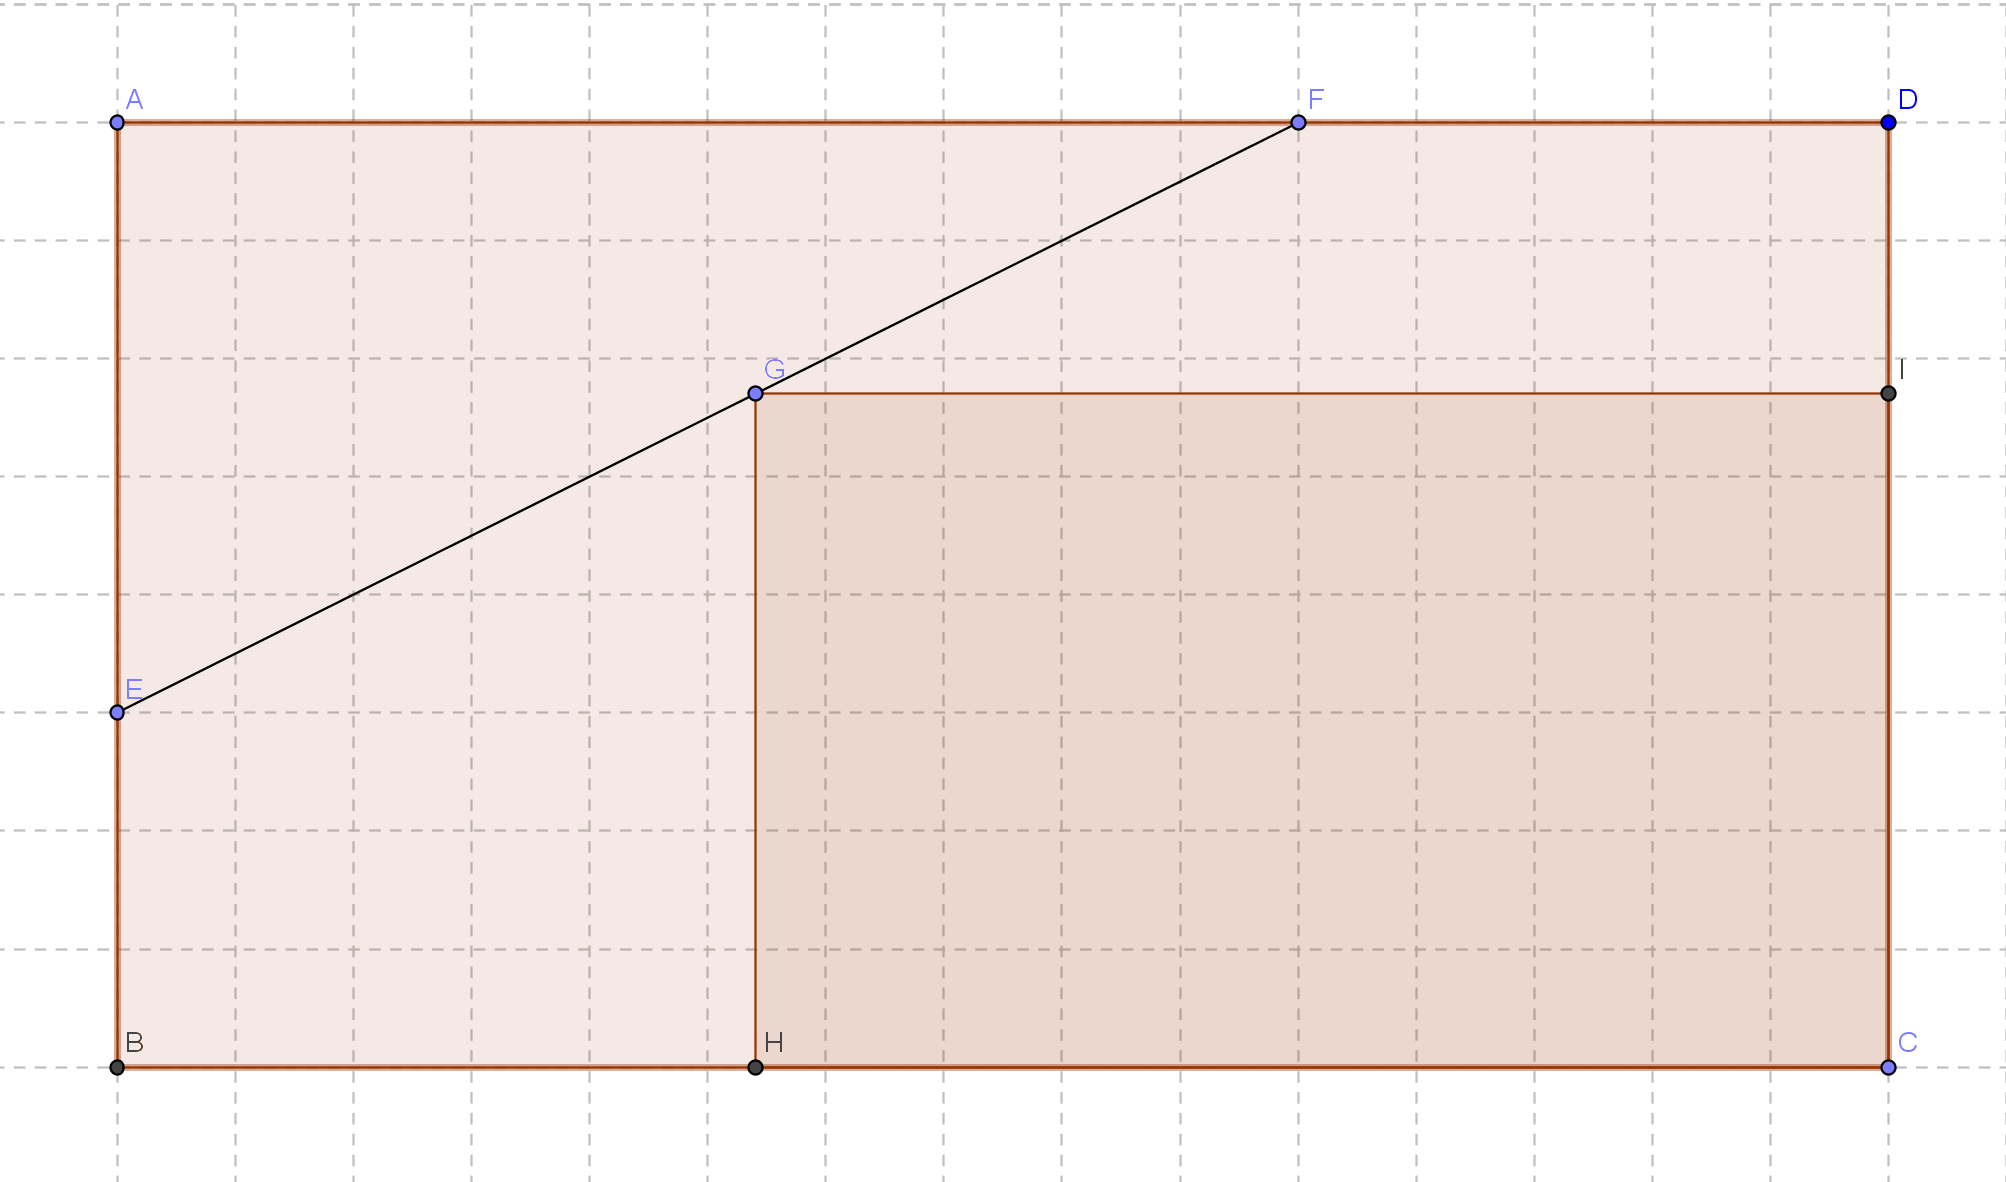
\includegraphics[width=0.7\textwidth]{problem_03}
\end{center}\medskip
\ep

\bp{04}
다음 그림과 같은 직사각형 ABCD에서 점 \(G\)가 \(\overline{EF}\) 위에서 움직일 때 직사각형 BHGI의 넓이의 최대값은?
(단 모눈 한 개의 눈금은 1이다.)
\par\medskip
\begin{center}
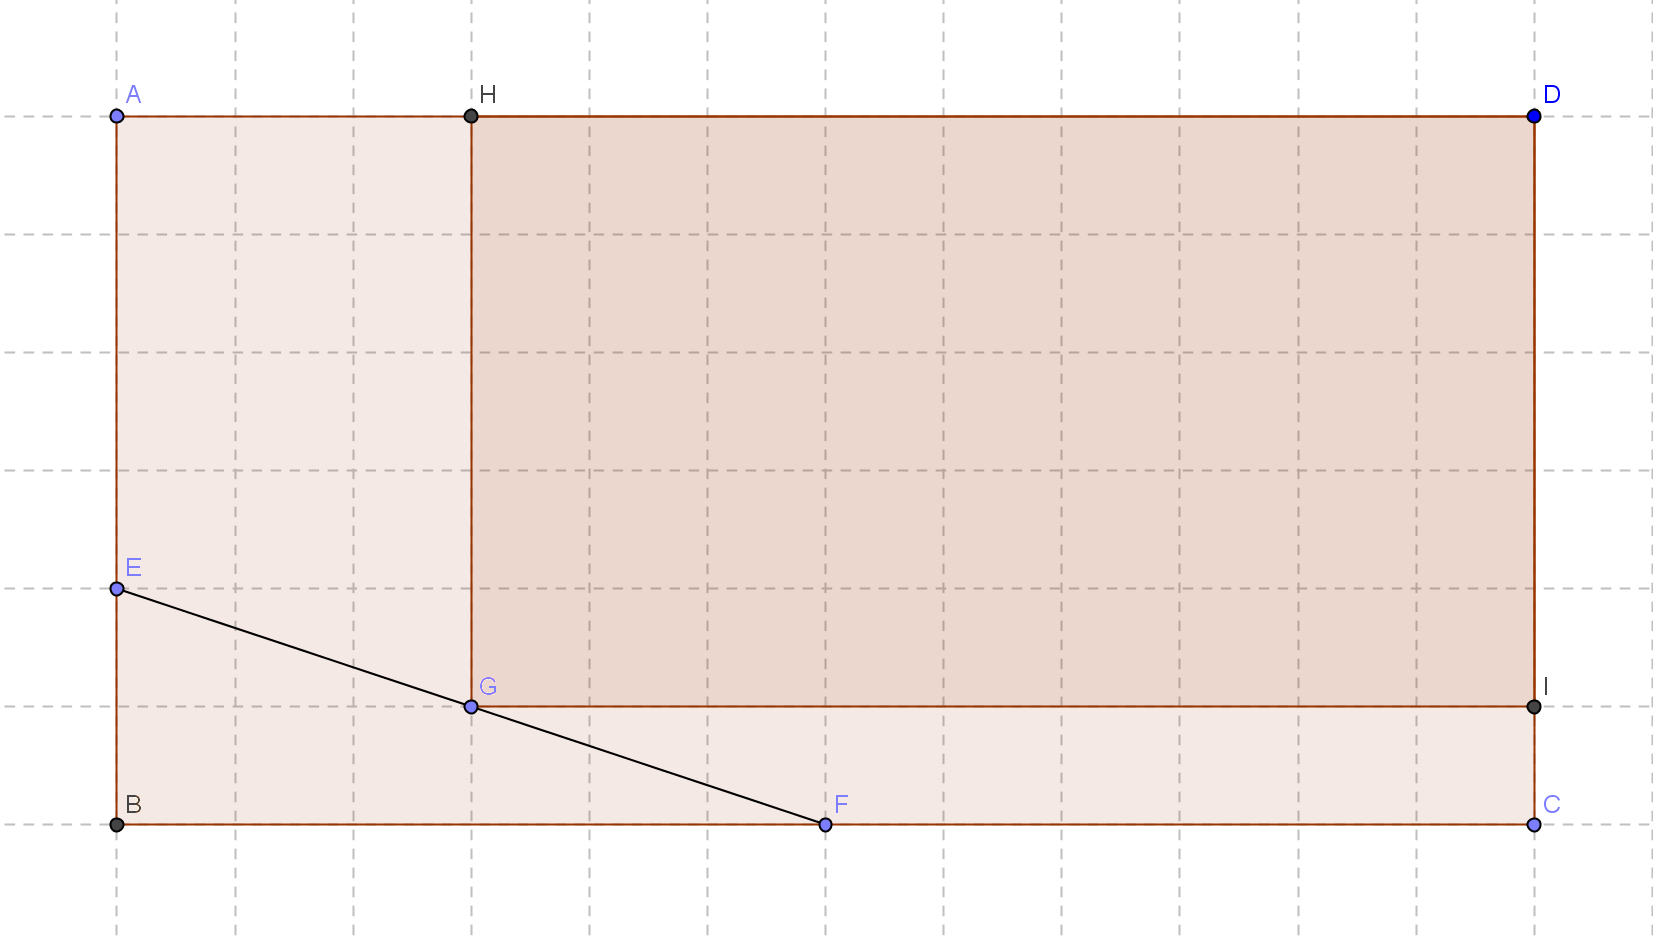
\includegraphics[width=0.7\textwidth]{problem_04}
\end{center}\medskip
\ep

\bp{05}
다음 그림과 같은 직사각형 ABCD에서 점 \(I\)가 \(\overline{GH}\) 위에서 움직이고 점 \(J\)는 \(\overline{EF}\) 위에서 움직일 때 직사각형 IJLK의 넓이의 최대값은?
(단 모눈 한 개의 눈금은 1이다.)
\par\medskip
\begin{center}
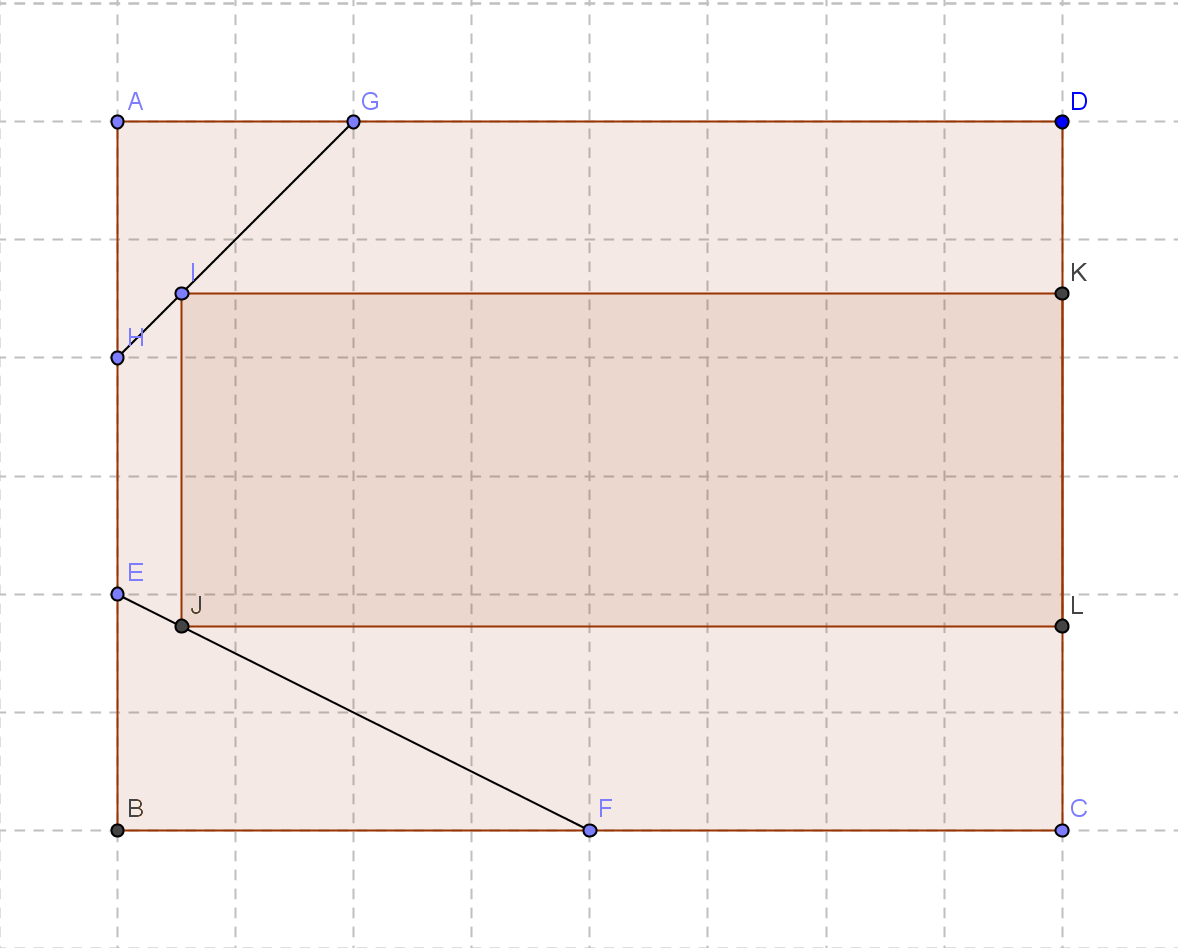
\includegraphics[width=0.7\textwidth]{problem_05}
\end{center}\medskip
\ep

\newpage
\section*{답}
01 : \(48\)\\
02 : \(54\)\\
03 : \\
04 : \(48\)\\
05 : 
\end{document}